
\documentclass[conference]{IEEEtran}
% If the IEEEtran.cls has not been installed into the LaTeX system files,
% manually specify the path to it: e.g.,
% \documentclass[conference]{../sty/IEEEtran}

\usepackage[latin1]{inputenc}
\usepackage{graphicx,color,longtable,multirow,times,float,eurosym,amsmath,url,subfigure}

% correct bad hyphenation here
\hyphenation{}

%\IEEEoverridecommandlockouts    % to create the author's affliation portion
                % using \thanks

%\textwidth 178mm    % <------ These are the adjustments we made 10/18/2005
%\textheight 239mm   % You may or may not need to adjust these numbes again
%\oddsidemargin -7mm
%\evensidemargin -7mm
%\topmargin -6mm
%\columnsep 5mm

\begin{document}


% paper title: Must keep \ \\ \LARGE\bf in it to leave enough margin.
\title{Towards a Multiobjective Evolutionary Approach to Inventory and Routing Management in a Retail Chain}

\author{\IEEEauthorblockN{A.I. Esparcia-Alcazar and A. Mart�nez-Garc�a}
\IEEEauthorblockA{S2 Grupo, Spain\\
Email: \{aesparcia,amartinez\}@s2grupo.es}
\and
\IEEEauthorblockN{P. Garc�a-S�nchez, J.J. Merelo and  A.M. Mora}
\IEEEauthorblockA{Depto. Arquitectura y Tecnolog\'ia de Computadores \\
University of Granada, Spain\\
Email: \{pgarcia,jmerelo,amorag\}@geneura.ugr.es}}

% author names and affiliations
% use a multiple column layout for up to three different
% affiliations
%\author{\IEEEauthorblockN{Juan-J. Merelo,  Antonio M. Mora \\ and Pedro Castillo}
%\IEEEauthorblockA{Departamento de Arquitectura y Tecnolog\'ia de Computadores \\
%University of Granada\\
%Email: \{jmerelo,amorag,pedro\}@geneura.ugr.es}
%\and
%\IEEEauthorblockN{Carlos Cotta}
%\IEEEauthorblockA{Departamento de Lenguajes y Ciencias de la Computaci\'on\\
%Universidad de M\'alaga\\
%Email: ccottap@lcc.uma.es}
%\and
%\IEEEauthorblockN{Mario Valdez}
%\IEEEauthorblockA{Instituto Tecnol�gico de Tijuana\\
%Tijuana, M�xico\\
%Email: mario@tectijuana.edu.mx}
%}

% make the title area
\maketitle

%
%%%%%%%%%%%%%%%%%%%%%%%%%%%%%%%   ABSTRACT   %%%%%%%%%%%%%%%%%%%%%%%%%%%%%%%
%
\begin{abstract}
In this work we address the problem of inventory and routing management in a retail chain. This involves the minimisation of two contradicting objectives, inventory holding costs and transportation costs, but which can be compounded in to a single one, the global costs. In previous work we addressed this using a single objective evolutionary algorithm but the duality inherent in the problem prompts us to consider a multiobjective approach; the aim is to determine what advantages each can bring. A number of experiments are carried out on several simulated and one real retail chain.
\end{abstract}

%
%%%%%%%%%%%%%%%%%%%%%%%%%%%%%%%   INTRODUCTION   %%%%%%%%%%%%%%%%%%%%%%%%%%%%%%%
%
\section{Introduction}
\label{sec:intro}
%

Inventory and Routing Problems (IRPs) are the most interesting and
challenging extensions to the classical vehicle routing problem
(VRP). In these problems inventory control and routing decisions
have to be made simultaneously. IRPs share in general two
characteristics: (1) either the supplier or the customer has a
limited storage capacity and (2) inventory holding costs may be
incurred, either at the supplier's or customer's end, which must be
taken into account \cite{bertazziSavelsberhSperanza2008}. IRPs are
more recent (dating back to the late 1970's, see for instance
\cite{conwhy78}) than the Vehicle Routing Problem (VRP) and differ
from it in several aspects. Firstly, in the VRP the customers place
orders and the delivery company serves them on any given day; in the
IRP problem, however, there are no customer orders and the delivery
company decides how much to deliver to which customers each day
\cite{campbellClarkSavelsbergh2002}. Another difference is the
planning horizon, which typically spans a single day for the VRP,
being longer for the IRP. Typically, an IRP aims to find an answer
to three issues: (1)~When to deliver to each customer (2)~How
much to deliver to a customer each time it is served and (3)~Which
delivery routes to use.

In general, IRPs are defined on a graph $G = (V, E)$, where
$V=\{S,1,\ldots,n\}$ is the set of vertices and $E$ is the set of
edges (or arcs). Vertex $S$ represents the supplier and vertices
$1\ldots n$ represent the customers. A travel time $t_{i,j}$ and a
cost $c_{i,j}$ are associated with edge $(i,j)\in E$. A time window
$[a_i, b_i]$ and a
service time $s_i$ are associated with each vertex $i \in V$. %\cite{cordesdessolsou2002}
The capacity of each vehicle is denoted by $Q$. The inventory holding cost at
the supplier is $h_S$ and at customer $i$ is $h_i$. The length of
the planning horizon is denoted by $H$. Vehicles are denoted by $k
\in K$. Other variables that can be considered are the initial
inventories at supplier and customers and rates of usage of goods.
% 1. ¿Por qué pones esto ahora, sin fórmula a la que agarrarse?
% 2. esta última frase sobra - JJ
% 1.- La formula viene enseguida
% 2.- Tampoco molesta mucho. Si necesito una linea mas la quitaré - Anna

Many variants of the IRP have been described in the literature, e.g.
\cite{ben89,buhabluda85}, some of which have referred to the
specific case of retail chains \cite{wallerJohnsonDavis1999}. Among
these versions some have been addressed using metaheuristics such as
PSO \cite{chenLin2009}, tabu search \cite{cousineau-ouimet2002} or
evolutionary algorithms \cite{EVITAchapter2008}. We will follow this
latter work and address here a variant of the Inventory Routing
Problem for the real case of a Spanish cosmetics retail chain, which
was first introduced in \cite{manolojosepe}. In this problem variant
the customers are the shops in the chain and the deliverer is a
central depot, all of them belonging to the same company. Added
features of the problem, as imposed by the company, are as follows:
\begin{itemize}
\item The planning horizon $H$ is one week, weekend excluded.
\item Inventory costs are considered for the whole planning horizon and only at the shops' end,  $h_S = 0$.
\item Each shop $i$ has a set of \emph{admissible delivery frequencies}, $F_i$, denoting the number of times a week they can be served.
\item For a given delivery frequency only certain combinations of days, or \emph{delivery patterns}, are admissible. The set of admissible patterns $\mathcal{P}_{adm}$is common to all shops.
\item The load is measured in units called \emph{roll containers}. A roll container is a sort of tall cage with
    wheels that can store many kinds of items. Hence, although there
    are thousands of different items we will consider them only as
    part of a homogeneous, discrete load.
\item For each shop and delivery frequency, the chain management has
  established an amount to deliver, expressed in roll
  containers. The question ``how much to
  deliver'' is thus simplified.
    \item The delivery fleet is homogeneous and capacitated (i.e. all vehicles used have the same finite capacity $Q$). The number of vehicles (i.e. the size of $K$) is not restricted. This is a consequence of the transport being subcontracted.
    \item All routes start and finish in the depot; each shop must be served once a day maximum.
    \item The service time is zero for the depot and the same value $s$ for the shops. There are no time
    windows.
\end{itemize}
The inventory holding costs, $c_h$, are thus calculated as follows:
\begin{eqnarray}\label{eqn:inventory_costs}
 c_h = \sum_{i\in V} h_i
\end{eqnarray}
and the transportation (delivery) costs, $c_t$,
\begin{eqnarray}\label{eqn:transport_costs}
c_t =  \sum_H \sum_{k \in K} \sum_{(i,i)\in E} c_{i,j}x_{ijk}
\end{eqnarray}
where the flow variable $x_{ijk}$ equals 1 if edge $(i,j)$ was used
by vehicle $k$ and 0 otherwise. The global costs are calculated as
the sum of the inventory costs and the transportation costs,
\begin{eqnarray}\label{eqn:singleobjective}
c_g =  c_h + c_t
\end{eqnarray}
and the goal is to \emph{minimise} $c_g$.% No habr�a que decir aqu��
                                % que hay que tener en cuenta las
                                % restricciones, porque todas las
                                % rutas no son posibles ? - JJ
                                % Yo creo que �a va sans dire, no? - Anna

The key issue in our problem is that the delivery frequency
determines the size of the deliveries, which in turn determine the
inventory cost at the shop's end. A low frequency of delivery
implies a large size of deliveries and a high inventory cost, and
vice-versa. On the other hand, a low delivery frequency also means
low transportation costs. Hence, the minimisation of inventory and
transportation costs are contradicting, independent
objectives, although it is true that they are both measured in the same (currency) units and that the global
cost is calculated by simply adding them.

The purpose of this work is to  explore the interest of applying a multiobjective approach to this seemingly monoobjective problem. The rationale behind this is that the search space will be explored in a different way and this may lead to novel results.  This problem has been previously addressed \cite{EVITAchapter2008} employing a two-level methodology in which
each level aimed at minimising each objective. The top level used an
evolutionary algorithm to obtain delivery patterns for each shop on
a weekly basis so as to minimise the inventory costs, while the
bottom level used various metaheuristics to solve the Capacitated
Vehicle Routing Problem (CVRP) for every day in order to obtain the
minimum transportation costs associated to a particular set of
patterns.

Here we have carried out an extensive series of
experiments using the eight instances used in
that work, plus three new ones (see Table
\ref{tab:problem_instances}). These correspond to 10 simulated geographical layouts found frequently in the literature, plus that of a real retail chain.
The set of restrictions, consisting of the characteristics of the
vehicles employed and the working hours of the drivers (see Table
\ref{tab:vehicledata}), plus the parameter configuration of the
evolutionary algorithm those used in \cite{EVITAchapter2008}. In the
multiobjective approach we have used the NSGA-II algorithm
 \cite{nsgaII2000} because it is considered one of the best algorithms in the state of the art.


The rest of the paper is structured as follows. The next section is devoted to briefly introduce the main concepts of multiobjective optimization. Delivery patterns are explained in Section \ref{sec:admpat}. The  methodology is
described in Section \ref{sec:evita}. Section \ref{sec:exp-simulated} describes the experimental setup with the simulated data, with results contained in Section \ref{sec:results_sim}. Section \ref{sec:exp-real} describes the experiments with real geographical data. Finally, Section \ref{sec:conclusions}
presents the conclusions and outlines future areas of research.
\begin{table}[hbt]
\begin{center}\setlength{\tabcolsep}{2mm}\caption{\label{tab:patterns}The
admissible patterns and their respective frequencies. The 1
represents that the shop is served on that day, the 0 that it is
not. As a consequence of the business logic, we will only consider
11 patterns out of the 31 that are possible.} {\scriptsize
\begin{tabular}  {ccccccc}  \multicolumn{7}{c}{}\\\hline
 \textbf{\scriptsize Pattern Id.}& \textbf{\scriptsize Freq. (days)} &\textbf{\scriptsize Mon}   & \textbf{\scriptsize Tues}  & \textbf{\scriptsize Wed}  & \textbf{\scriptsize Thurs}  & \textbf{\scriptsize Fri} \\
\hline
5 &2& 0 &0 & 1 & 0 & 1  \\
9 &2& 0 & 1  &0 & 0& 1 \\
10 &2& 0 & 1 &0 &  1  &0\\
11 &3& 0 & 1  &0 &  1  & 1  \\
13 &3& 0 & 1  & 1 & 0 & 1 \\
17 &2&  1  &0 &0& 0 & 1  \\
18 &2&  1  &0 &0 &  1 & 0 \\
21 &3&  1  &0 & 1  & 0 & 1  \\
23&4&  1  &0 & 1  &  1  & 1  \\
29&4&  1  & 1  & 1  & 0 & 1  \\
31&5&  1  & 1  & 1  &  1  & 1 \\
\hline \multicolumn{7}{c}{} \\
\end{tabular}} \end{center}
\end{table}

%%%%%%%%%%%%%%%%%%%%%%%%%%%%  MO Optimization  %%%%%%%%%%%%%%%%%%%%%%%%%%%%%%%%

\section{Multiobjective optimization}
\label{sec:mulobj}

Multicriteria or Multiobjective Optimization Problems\\ (MOP)
\cite{Osyczka1985} are those where several 
 objectives have to be simultaneously optimized. These problems do not
 have a single best solution, one that is better than any other with
 respect to every objective. In fact, frequently improving the
 solution for one objective implies a worsening for another. 
%
Thus in a MOP there is a set of solutions that are better than the rest considering all the objectives; this set is known as the \textit{Pareto set} (PS). They try to approach the ideal set of solutions
which is usually represented graphically as the \textit{Pareto front} (PF). These are related to an important concept, the \textit{dominance}, defined as follows (\textit{a} dominates \textit{b}):
%
\begin{small}
\begin{equation}\label{eq:modom}
\begin{array}{ll}
a \prec b\;\;if: \\
\forall i\in 1,2,...,k \; | \; C_i(a)\leq C_i(b)\:\; \wedge \:\; \exists j\in 1,2,...k \;| \; C_j(a)<C_j(b)
\end{array}
\end{equation}
\end{small}
%
where \textit{a $\in$ X} and \textit{b $\in$ X} are two different decision vectors of \textit{n} values, and every \textit{C} is a cost function (one per objective). If it intends to minimize the cost and Equation \ref{eq:modom} is true, then \textit{b is dominated by a}.

Hence, the solutions in the PS are known as \textit{non-dominated solutions}, while the remainder are known as dominated solutions. 
%
%Figure \ref{fig:pareto_front} shows the representation of the PF of a multi-objective (bi-criteria) problem, where the domination concept can be clearly seen.
%
%\begin{figure}[ht]
%\begin{center}
%\includegraphics[scale=0.5]{figures/pareto_front.eps}
%\caption{Example of the Pareto front in a problem with two objectives to minimize (F1 and F2). Black dots correspond to solutions in the Pareto front ($a$ and $b$ among them). Dominated solutions are shown in gray ($c$ for instance).
%\label{fig:pareto_front}}
%\end{center}
%\end{figure}
%
Since none of the solutions in the PS is absolutely better
than the other non-dominated solutions, all of them are equally
acceptable as regards the satisfaction of all the objectives. These concepts can be extended in \cite{Coello2002}. 


%%%%%%%%%%%%%%%%%%%%%%%%%%%%%  Admisible Patterns  %%%%%%%%%%%%%%%%%%%%%%%%%%%%%

\section{Admissible patterns}
\label{sec:admpat}

A delivery pattern is a set of days in the week in which a shop can
be served. It can be represented by $d$ bits, with a bit set to one
meaning that the shop is visited that day and nil that it is not.
For instance, pattern 21, i.e. 10101 in binary, corresponds to
deliveries on Monday, Wednesday and Friday. The total number of
possible patterns is $2^d -1$, in our case $2^5-1= 31$ (obviously
pattern 0 does not make sense, as it would involve not serving any
day). However, not all patterns are acceptable from a business point
of view. For instance, no patterns of frequency 1 (serving one day a
week) are admissible, because this would involve big deliveries
which would interfere with the shop staff's main activity of
selling. Furthermore, delivery patterns that involve serving only
Monday and Tuesday are not admissible, as most sales take place
towards the end of the week. Hence, for a pattern $p_i$ to be valid
it must be contained in the set of admissible patterns, $p_i \in$  $\mathcal{P}_{adm}$ or as given in Table \ref{tab:patterns}.


As a pattern has an associated delivery frequency and only a limited
number of frequencies are available to each shop, this in turn means
that the number of patterns available to a shop can be very low. For
instance, a shop whose admissible frequencies are 4 and 5 has only
three possible patterns: 23, 29 and 31.


%%%%%%%%%%%%%%%%%%%%%%%%%%%%%%  METHODOLOGY  %%%%%%%%%%%%%%%%%%%%%%%%%%%%%%
%
\section{Methodology}
\label{sec:evita}

Following \cite{EVITAchapter2008} we have employed an evolutionary
algorithm (see details in Table \ref{tab:evopars-toplevel}) with each individual being a set of patterns $\mathcal{P}$ represented as a vector of length
equal to the number of shops to serve, ($n$),

\[ P = ( p_1, p_2, \ldots, p_n) \]

\noindent with $p_i \in$ $\mathcal{P}_{adm}$.

To calculate the inventory cost for such an individual we first obtain the inventory cost $h_i$ for each shop $i$. This stems from the
shop's pattern, which in turn determines the associated delivery
frequency for that shop. With this value we would read the inventory cost for that shop in the
corresponding table. An example of the latter is given in Table
\ref{tab:inventorycost}.


\begin{table}[htb]
\begin{center}\setlength{\tabcolsep}{0.7mm}\caption{\label{tab:inventorycost}Inventory cost (in Euro) and size of the deliveries per shop (expressed in roll containers) depending on the delivery frequency (in days). Missing data corresponds to
frequencies that are not admissible for each shop.}% Shop number 0 corresponds to the depot. }
{\scriptsize
\begin{tabular} {c|ccccc|ccccc}
\multicolumn{11}{c}{ }\\
\hline\hline
    &   \multicolumn{5}{c|}{ }   &    \multicolumn{5}{c}{ }    \\
    &   \multicolumn{5}{c|}{Inventory cost }   &    \multicolumn{5}{c}{Delivery size}    \\
  &    \multicolumn{5}{c|}{(\euro)}           &   \multicolumn{5}{c}{{\scriptsize(roll containers)}}  \\%\cline{2-11}
 &    \multicolumn{5}{c|}{}                                   &   \multicolumn{5}{c}{}\\
 Shop  \#& \multicolumn{5}{c|}{{\scriptsize Frequency (days)} } & \multicolumn{5}{c}{{\scriptsize Frequency (days)} }\\
%\hline \\
  &   1   &   2   &   3   &   4   &   5   &   1   &   2   &   3   &   4   &   5      \\
\hline
1   &   - &   - &   - &   336 &   325 &   -   &   -   &   -   &   2   &   2      \\
2   &   - &   - &   - &   335 &   325 &   -   &   -   &   -   &   2   &   2  \\
 $\cdots$   &   $\cdots$ &    $\cdots$ &    $\cdots$ &    $\cdots$ &    $\cdots$ &    $\cdots$   &    $\cdots$   &    $\cdots$   &    $\cdots$   &  \\
N  &   - &   311 &   293 &   286 &   284 &   -   &   3   &   2   &   2   &   1   \\
\hline\hline \multicolumn{11}{c}{ }\\
\end{tabular} }
\end{center}
\end{table}

For instance, let us assume that shop N was assigned pattern 23, which has a
frequency of 4; we would look up in the table the inventory cost for
the shop at that frequency, which is 286\euro. Proceeding in the
same way with all shops and adding up the results we would obtain
the total inventory cost.

\begin{table*}[tb]
\begin{center}\setlength{\tabcolsep}{2mm}
\renewcommand{\arraystretch}{1.3}
\caption{\label{tab:evopars-toplevel}Configuration of the top-level
evolutionary algorithm employed (both mono- and multiobjective).}
{\scriptsize
%{\footnotesize
\begin{tabular}{lp{8.5cm}} \multicolumn{2}{c}{}\\\hline
\textbf{Encoding} & The gene $i$ represents the pattern for shop
$i$.\\
&The chromosome length is equal to the number of shops
($n$).\\
 \textbf{Selection} & Tournament
in 2 steps. To select each parent, we take $tSize$ individuals
chosen randomly and select the best.\\
& For the single objective algorithm the best 10 individuals of each
generation are preserved as the
elite.\\
\textbf{Evolutionary operators} & 2 point crossover and 1-point
mutation. \\
& The mutation operator changes the pattern for
1 shop in the chromosome.  \\
 \textbf{Termination criterion}& Terminate when the total number of generations (including the initial one) equals 100.\\
\textbf{Fixed parameters} & Population size, $popSize =100$\\
& Tournament size, $tSize = 2$\\
& Mutation probability, $pM = 0.2$ \\
& Crossover probability, $pC = 1$ \\\hline
\multicolumn{2}{c}{}\\
\end{tabular}}
\end{center}
\end{table*}

The next step involves the calculation of transport costs,
which are obtained by solving the VRP with an algorithm of choice.
In our case we will employ the one that yielded better results in
\cite{EVITAchapter2008}, namely the Clark and Wright algorithm
\cite{clawri64} enhanced with local search. C\&W's algorithm  is
based on the concept of \emph{saving}, which is the reduction in the
traveled length achieved when combining two routes. The local search method implemented  consists on
performing 2-interchanges on the  solution obtained by the C\&W
algorithm. Every possible pair of shops is exchanged, first between
shops in the same route and then between shops in different routes.
If at any time an invalid route is generated (because the
restrictions on time or capacity are violated) the depot is inserted
where required in the route. The best neighbour solution will be the
one with a lower associated transport cost.

Because we are dealing with the \emph{capacitated} VRP, we need to know what the demands (i.e. the size of deliveries) of each shop are. These are  taken from Table \ref{tab:inventorycost}. In the example given earlier, for shop N at frequency 4 the delivery size is 2 roll containers.

Having established the inventory and routing costs, we need to define what the optimum is. In the single objective case, this is defined as the solution that minimises the global cost, given by Equation
(\ref{eqn:singleobjective}). In the multiple objective approach, we
will deal with two separate cost functions, given by Equations
(\ref{eqn:inventory_costs}) and (\ref{eqn:transport_costs}).
However, in the latter case we will still use the global cost
defined for the single objective case to compare the results between
multi and monoobjective solutions. The reason is that the company is
interested in spending less, irrespective of where the reduction
comes from, and in any case both costs come in the same units
(\euro).
\begin{table}[hbt]
\begin{center}
\caption{ \label{tab:problem_instances}Problem instances used in the experiments and their characteristics. All instances were obtained from \texttt{branchandcut.org/VRP/data/} except the last one, which was obtained from \texttt{www.fernuni-hagen.de/WINF/touren/inhalte/} \texttt{prob-inst.htm}}
\setlength{\tabcolsep}{1.5mm}{\scriptsize
\begin{tabular} {llcccl}
\multicolumn{6}{c}{ }\\
\hline
\textbf{ID}  &   \textbf{Instance}    &   \textbf{Distribution }   &   $n$    &   \textbf{Eccentricity} & \textbf{Source}    \\
\hline
A32 &   A-n32-k5.vrp    &   uniform  &   31 &   0.370 & Branchandcut \\
A33 &   A-n33-k5.vrp    &   uniform  &   32 &   0.173 & Branchandcut \\
A69 &   A-n69-k9.vrp    &   uniform  &   68 &   0.124 & Branchandcut \\
A80 &   A-n80-k10.vrp   &   uniform  &   79 &   0.460 & Branchandcut \\
B35 &   B-n35-k5.vrp    &   clusters &   34 &   0.518 & Branchandcut \\
B45 &   B-n45-k5.vrp    &   clusters &   44 &   0.128 & Branchandcut \\
B67 &   B-n67-k10.vrp   &   clusters &   66 &   0.163 & Branchandcut \\
B68 &   B-n68-k9.vrp    &   clusters &   67 &   0.468 & Branchandcut \\
P100&   P-n101-k4.vrp   &   uniform  &  100 &   0.017 & Branchandcut \\
X200&   c1\_2\_1.txt    &   clusters &  200 &   0.043 & Uni. Hagen\\
\hline
\multicolumn{5}{c}{ }\\
\end{tabular}}
\end{center}\end{table}


%%%%%%%%%%%%%%%%%%%%%%%%%%%%%%%   EXPERIMENTS  %%%%%%%%%%%%%%%%%%%%%%%%%%%%%%%%
%
\section{Experiments with simulated data}\label{sec:exp-simulated}

%This section is devoted to present the data we have used in the
%problem (subsection \ref{subsec:data}) and the experimental
%procedure we have followed (in the next subsection,
%\ref{subsec:exp-procedure}).

%\subsection{Problem data} \label{subsec:data}

As explained above, we have employed a number of \emph{geographical
layouts} available on the web. We have selected our instances so as
to achieve the maximum representation on three
categories:\begin{itemize}
\item{\textbf{size}, given by the number of shops, $n$,}
\item{\textbf{distribution}. We consider two kinds of distributions:
\emph{uniform} and \emph{in clusters}, corresponding to shops that
are scattered more or less uniformly on the map or grouped in
clusters and,}
\item{\textbf{eccentricity}. This represents the distance
between the depot and the geographical center of the distribution of
shops, normalised by dividing it by the maximum distance between any two points in the geographical distribution. The coordinates of the geographical center are calculated as
follows: \begin{equation*}
(x_{gc} ,y_{gc}) = \frac{1}{n}\sum_{i=1}^{n} (x_i,y_i) %\\
\end{equation*} with $n$ being the number of shops. An instance with low eccentricity (in practise, less than
0.15) would have the depot centered in the middle of the shops while
in another with high eccentricity (above 0.35) most shops would be
located on one side of the depot.}\end{itemize}
\begin{table}[tbh]
\begin{center}\setlength{\tabcolsep}{2mm}\caption{\label{tab:vehicledata}Data for Vehicle Routing Problem}%{\footnotesize
\begin{tabular} {ll} \multicolumn{2}{c}{} \\   \hline

\textbf{Vehicle capacity}    & 12 roll containers\\
\textbf{Transportation cost} &    0.6 \euro /Km \\ %\hline \hline
\textbf{Average speed}  & 60 km/h \\
\textbf{Unloading time}  & 15 min  \\
\textbf{Maximum working time} &8h\\
\hline
 \multicolumn{2}{c}{ }\\
\end{tabular}%}
\end{center}
\end{table}
We chose ten instances with different levels of each category, see
Table \ref{tab:problem_instances}. It must be noted that we are only
using the spatial location and not other restrictions given in the
bibliography, such as the number of vehicles  or the shop demand
values. As pointed out earlier, a main characteristic of our problem
is that the latter is a function of the delivery frequency, so we
had to use our own values for the demands. We also added the set of
admissible patterns
$\mathcal{P}_{adm}=\{5,9,10,11,13,17,18,21,23,29,31\}$  and the
inventory costs, an example of which is given in Table
\ref{tab:inventorycost}. The inventory, demand and admissible
patterns data were obtained from Druni SA, \url{http://www.druni.es}, a major regional Spanish
drugstore chain. Finally, we used the vehicle data given in Table
\ref{tab:vehicledata}. Problem data is freely available from our
 website %\url{http://casnew.iti.es/}
\url{http://ourdata.repository.org}%\footnote{Its use is subject to the condition that this or other papers on the same subject by the authors are mentioned}

%In the original problem the $n$ indices represented the number of shops plus one and the $k$ indices the maximum number of vehicles
%allowed. In our case we will ignore the latter data, as we are not considering restrictions in the number of vehicles.

\begin{figure}[bhtp!]
\begin{center}
%\fbox{
\resizebox{6cm}{!}{
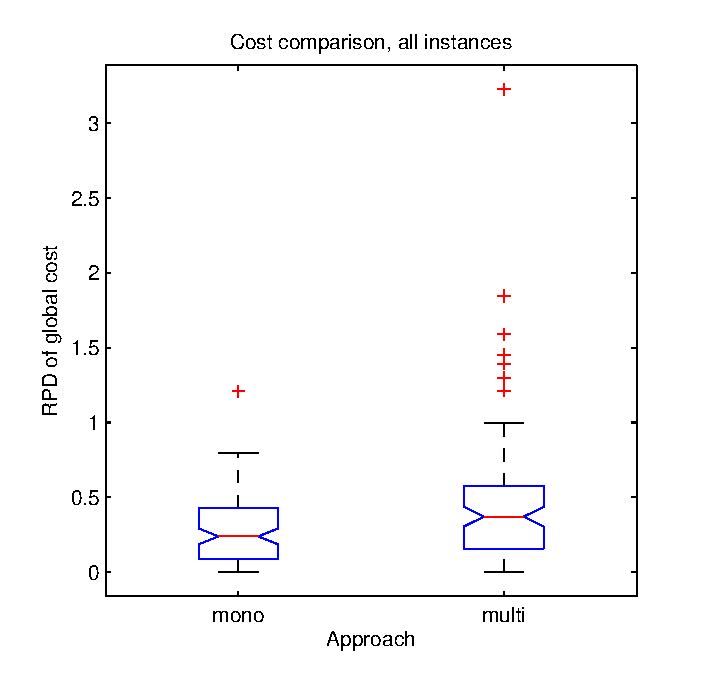
\includegraphics{figs/costcomparison.eps}}
\resizebox{6cm}{!}{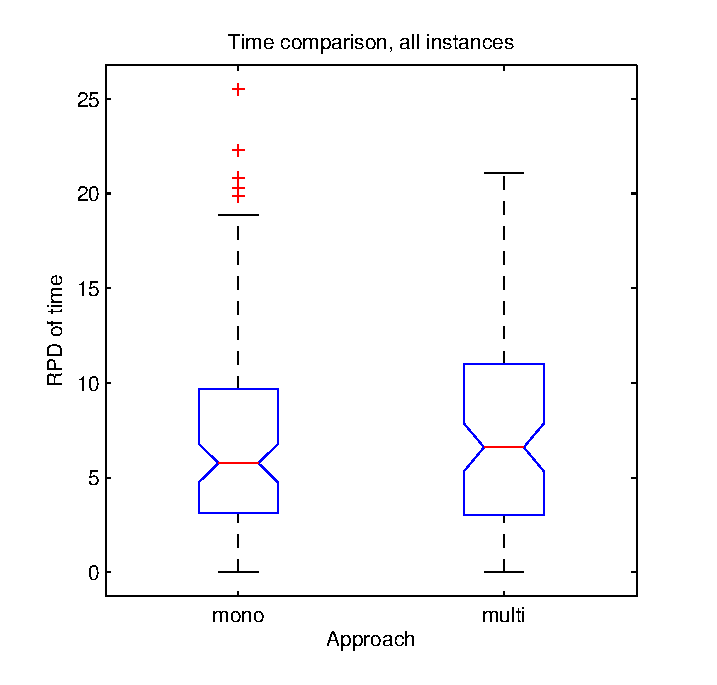
\includegraphics{figs/timecomparison.eps} }
\caption{\label{fig:boxplot-cost-and-time-comparison}\emph{Boxplots}
of RPDs of global costs and time for all instances.}
\end{center}
\end{figure}
We tested the mono- and
multiobjective approaches on each of the ten instances selected, performing ten runs per
instance with a termination criterion in all cases of 100
generations.\footnote{The motivation for such a small number of runs is the
high computational expense of some of the instances: the running times ranged from several minutes to several days in the
computers employed (PCs with  Intel Celeron processor, between 1 and 3GHz, between 256 and 512 MB RAM).}

The results were evaluated on two fronts: the global costs
obtained, and the computational time taken in the runs. The latter
is important when considering a possible commercial application of
the proposed methodology in a decision making environment, where answers to
queries must come as fast as possible.

%%%%%%%%%%%%%%%%%%%%%%%%%%%%%%%% RESULTS %%%%%%%%%%%%%%%%%%%%%%%%%%%%%%%

\section{Results with simulated data}\label{sec:results_sim}

In order to be able to compare results between the different
instances we normalised the values of interest by defining the
\emph{relative percentage deviation}, $RPD$, given by the following
expression:
%

\begin{equation}\label{eqn:RPD}
RPD = \frac{val - val_{min}}{val_{min}} \times 100
\end{equation}

%
\noindent where $val$ is the value of the variable of interest
obtained by EVITA using one of the two approaches (single or
multiobjective) on a given instance. The $RPD$ is, therefore, the
average percentage increase over the lower bound for each instance,
$val_{min}$. In our case, the values of interest are the
\textbf{cost} (global, inventory and transportation) and the
\textbf{execution time}. The lower bound is the best result obtained
for that instance.


We carried out Mann-Whitney-Wilcoxon (MWW) tests for the results
yielded by the best individuals for all runs and problem instances,
both in single and multiobjective. In the multiobjective case, we
define the best individual as that member of the final Pareto front
yielding the lowest global cost (as defined for the single objective
problem). %The MWW test is a non-parametric test for two-sample
%comparisons which is suited to the case at hand, in which the number
%of runs performed for each instance is small. This test does not
%require normality or homoskedasticity, which are not guaranteed in
%our case.


Firstly we examined all instances together, both in terms of
cost (global, inventory and routing) and time.
\begin{figure*}[htbp!]
\begin{center}
\resizebox{6 cm}{!}{
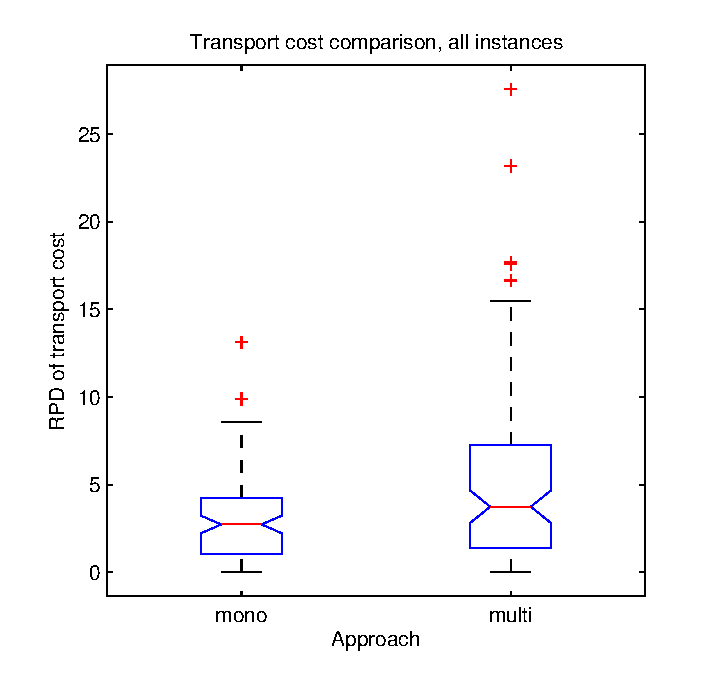
\includegraphics{figs/transportcomparison.eps}
} \resizebox{6cm}{!}{
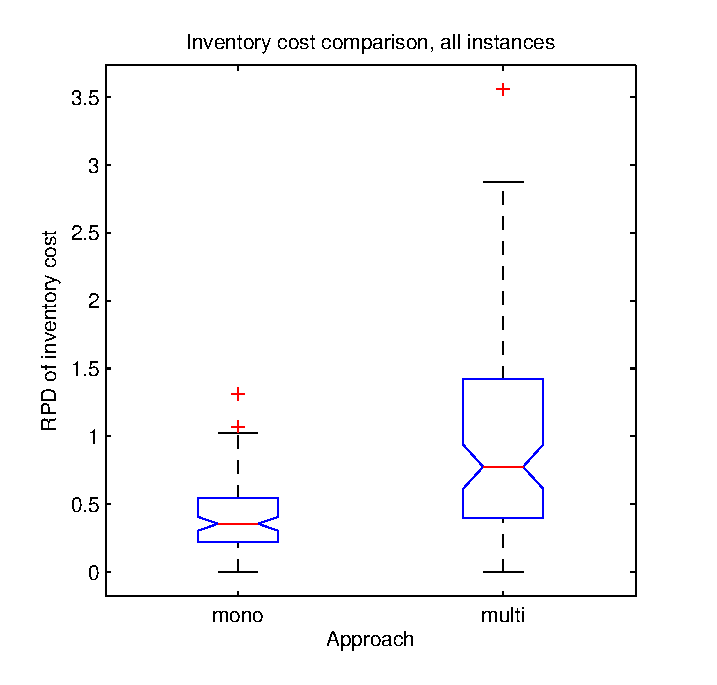
\includegraphics{figs/inventorycomparison.eps}
} \caption{\label{fig:inv_vs_transp}Boxplots for RPD of the transport
(left) and inventory costs (right) for all instances}
\end{center}
\end{figure*}
Next, we grouped the instances in several ways,
considering two levels in the three different categories:
\begin{itemize} \item Size: small
 (A32, A33, B35, B45) and large instances (A80, P100, X200)
 \item Distribution: uniform (A32, A33, A69, A80, P100) and clusters
 (B35, B45, B67, B68, X200)
 \item Eccentricity: low (P100, X200, A69, B45) and high (A80, B35,
 B68)\end{itemize}


The result of  the MWW tests is that the single
objective approach yields the best performance in terms of cost in
all cases but one, the low eccentricity group, for which there were
no significant differences.

\begin{figure}[htbp!]
\begin{center}
\resizebox{6cm}{!}{
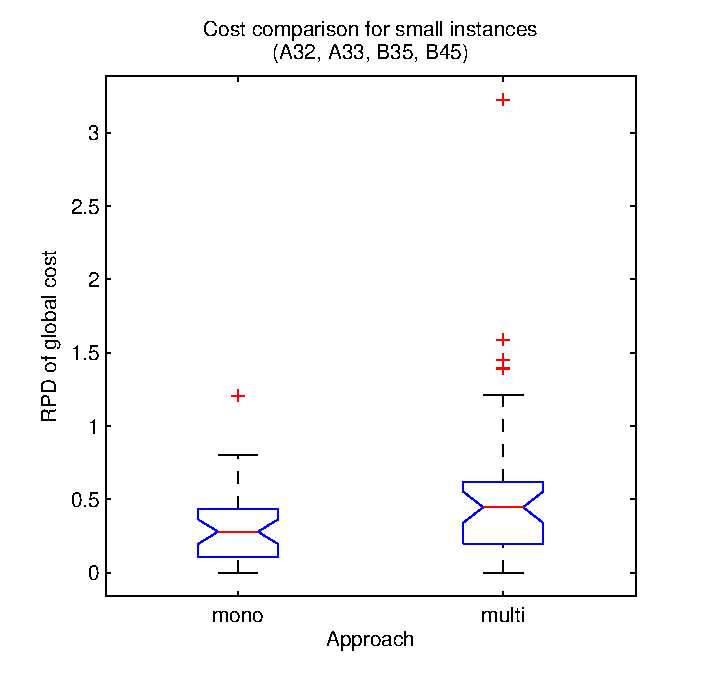
\includegraphics{figs/smallcomparison.eps}}
\resizebox{6cm}{!}{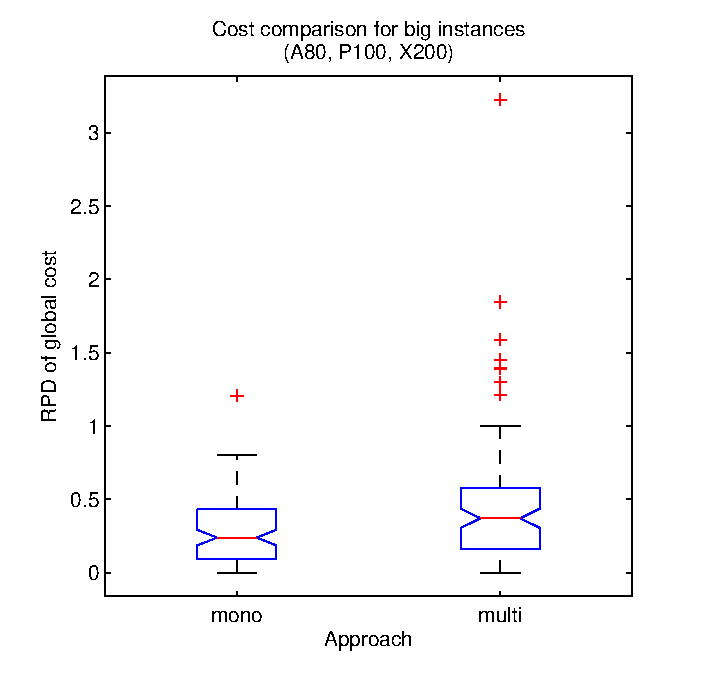
\includegraphics{figs/bigcomparison.eps}}
\caption{\label{fig:all-groups-comparison}\emph{Boxplots} of the RPD
of the global costs for large and small instances.}
\end{center}
\end{figure}

Regarding the computational time, the
test did not find any significant differences between the
two approaches. Figure \ref{fig:boxplot-cost-and-time-comparison} %and \ref{fig:boxplot-rareprobs}
shows the resulting boxplots for global cost and time for the ten
instances studied. Figure \ref{fig:inv_vs_transp} portrays the
comparison between methods when the costs of transport and inventory
are considered separately. Figure \ref{fig:all-groups-comparison}
shows the boxplots when different groupings by category are
considered.

\begin{figure}[htbp!]
\begin{center}
\resizebox{6cm}{!}{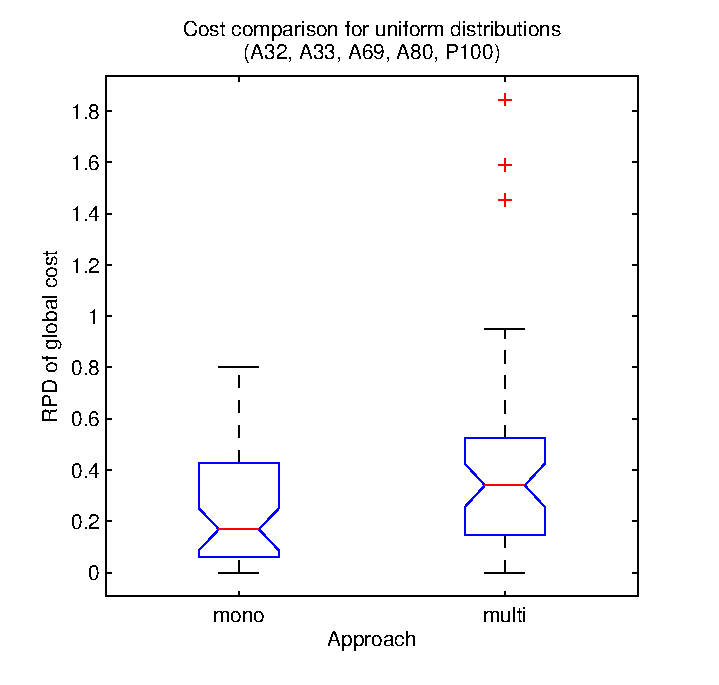
\includegraphics{figs/uniformcomparison.eps}}
\resizebox{6cm}{!}{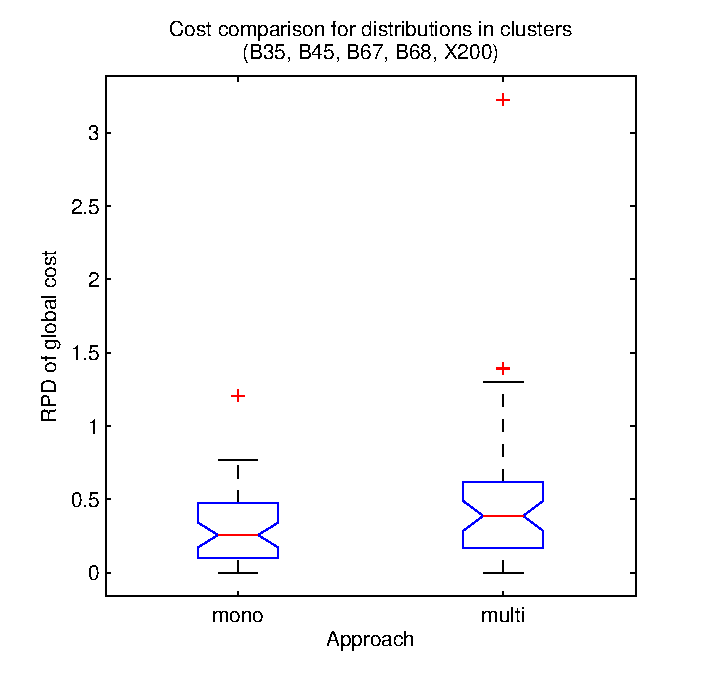
\includegraphics{figs/clusterscomparison.eps}}
\caption{\label{fig:all-groups-comparison2}\emph{Boxplots} of the RPD
of the global costs for instances with uniform and clustered distributions.}
\end{center}
\end{figure}

\section{Experiments with real geographical data}\label{sec:exp-real}
For this part we employed the geographical layout of the actual Druni stores. We restricted our problem to the 60 shops in the
province of Valencia (Spain), which make up a medium-sized instance when compared to the simulated instances of the previous sections. The distances between shops and between the depot and each shop were calculated using
Google Maps and therefore are not Euclidean but driving distances.
\begin{figure}[htbp!]
\begin{center}
\resizebox{6cm}{!}{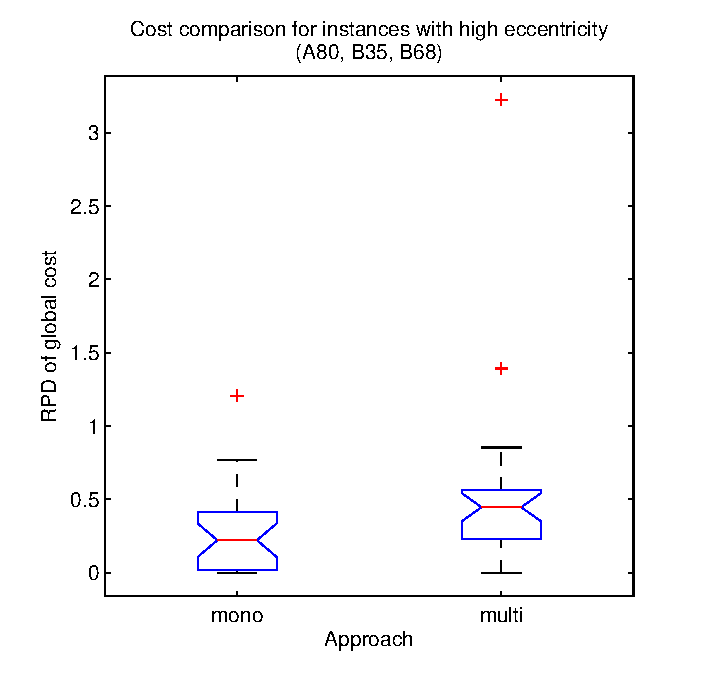
\includegraphics{figs/hiexcomparison.eps}}
\resizebox{6cm}{!}{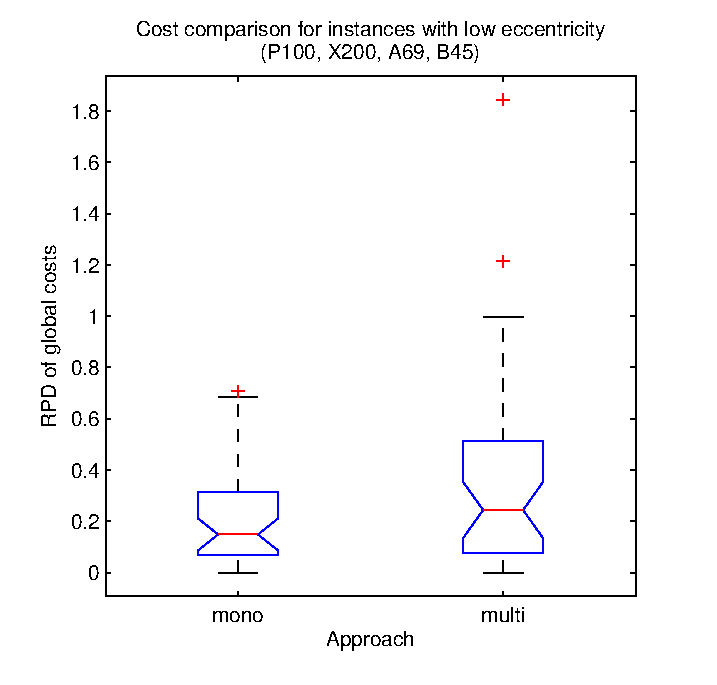
\includegraphics{figs/loexcomparison.eps}}
\caption{\label{fig:eccen-comparison}\emph{Boxplots} of the RPD
of the global costs for instances with high and low eccentricity.}
\end{center}
\end{figure}
 Figure
\ref{fig:shopsgeolayout} shows the geographical layout of the shops, taken from \url{http://maps.google.es/}.
The black dot marks the position of the depot. From this map we can see that the instance is not easily classifiable as having a uniform or clustered distribution.

\begin{figure}[htb]
\begin{center}
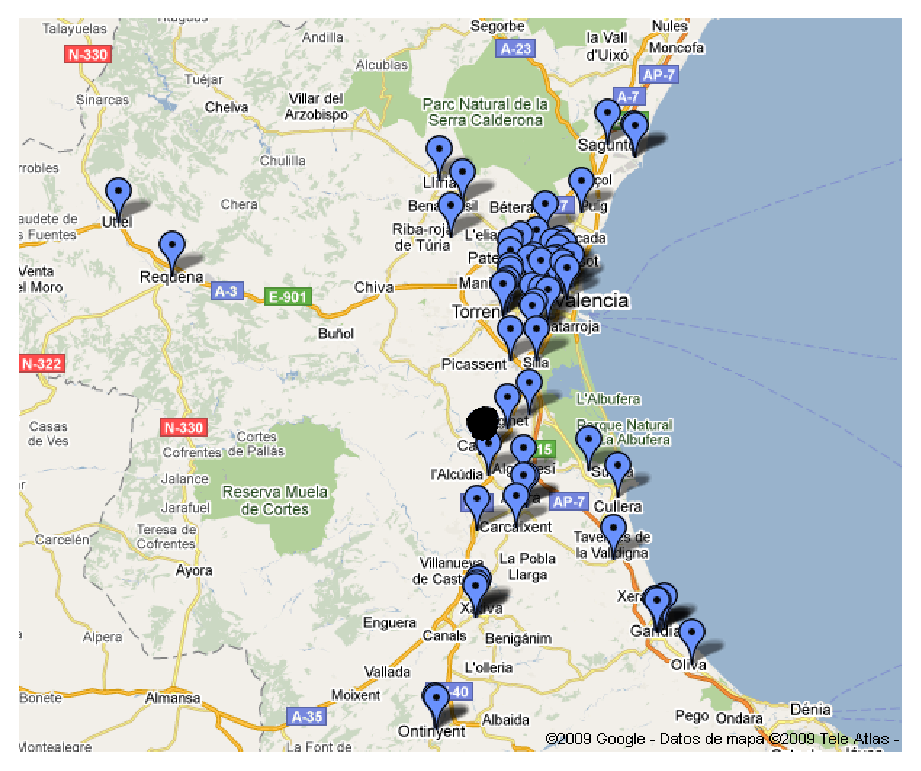
\includegraphics[scale=0.5]{figs/tiendasdruni.eps}
\caption{\label{fig:shopsgeolayout}Geographical layout of the shops. The black dot represents the depot.}
\end{center}
\end{figure}

We may also calculate the eccentricity of this distribution by calculating an approximated geographical center. For this, we will project the shops onto a plane and obtain their cartesian coordinates, which we will then use to obtain the center in the same way as for the simulated distributions.
The cartesian coordinates of shop $i$ expressed in kilometers are approximated as follows\footnote{We wish to thank A Friend for his help in nautical issues}:
\begin{eqnarray}\label{eqn:approx_coordinates}
y_i &=&  1.852 \cdot lat_i  \\
x_i &=& 1.852 \cdot long_i \cdot \cos(lat_i)
\end{eqnarray}
where $lat_i$ and $long_i$ are the latitude and longitude in minutes of shop $i$, respectively, and 1.852 is used to transform nautical miles into Km (taking into account that one minute of latitude is the length of a nautical mile). Employing this approximation we obtain an eccentricity of either 0.091 (employing Euclidean distance measure) or 0.113 (employing Google Maps driving distance); in both cases and according to the definition given in the previous section we can classify this as a low eccentricity setting, which is not unexpected given that this is a real retail chain.

Depending on their location, we consider seven types of shop, labeled A to G. We also used the list of admissible patterns defined in
Section \ref{sec:exp-simulated} and the inventory costs given in Table \ref{tab:inventorycost_Druni}. All the
problem data, including the table of driving distances, can be downloaded
from \url{http://ourdata.repository.org}.%\url{http://casnew.iti.upv.es/}


\begin{table}[htb]
\begin{center}\setlength{\tabcolsep}{1.2mm}\caption{\label{tab:inventorycost_Druni}Inventory cost (in \euro) and size of the deliveries per shop (expressed in roll containers) depending on the delivery frequency (in days). Missing data corresponds to
frequencies that are not admissible for each shop.}% Shop number 0 corresponds to the depot. }
{\scriptsize
\begin{tabular} {c|ccccc|ccccc}
\multicolumn{11}{c}{ }\\
\hline \hline
    &   \multicolumn{5}{c|}{ }   &    \multicolumn{5}{c}{ }    \\
    &   \multicolumn{5}{c|}{Inventory cost }   &    \multicolumn{5}{c}{Delivery size}    \\
  &    \multicolumn{5}{c|}{(euros)}           &   \multicolumn{5}{c}{{\scriptsize(roll containers)}}  \\%\cline{2-11}
 &    \multicolumn{5}{c|}{}                                   &   \multicolumn{5}{c}{}\\
 Shop  & \multicolumn{5}{c|}{{\scriptsize Frequency (days)} } & \multicolumn{5}{c}{{\scriptsize Frequency (days)} }\\
%\hline \\
type  &   1   &   2   &   3   &   4   &   5   &   1   &   2   &   3   &   4   &   5      \\
\hline
 &    \multicolumn{5}{c|}{}                                   &   \multicolumn{5}{c}{}\\
A   &   - &   - &   - &   336 &   325 &   -   &   -   &   -   &   2   &   2      \\
B   &   - &   - &   - &   327 &   317 &   -   &   -   &   -   &   2   &   2  \\
C   &   - &   330 &  311 &  303 &   301 &   -  &   4   &   2   &   2   &   1  \\
D   &   - &   310 &  292 &  285 &   283 &   -  &   3   &   2   &   2   &   1  \\
E   &   - &   293 &  276 &  269 &   267 &   -  &   3   &   2   &   2   &   1  \\
F   &   - &   277 &  261 &  255 &   - &   -   &   2   &   2   &   1   &   -  \\
G  &   - &   268 &   253 &   - &   - &   -   &   2   &   1   &   -   &   -   \\
\hline \hline \multicolumn{11}{c}{ }\\
\multicolumn{11}{l}{\textbf{Shop type codes}}\\ \multicolumn{11}{c}{ }\\
\multicolumn{6}{l}{A - Valencia city center }& \multicolumn{5}{l}{E - La Ribera county  }\\
\multicolumn{6}{l}{B - Valencia other + shopping malls}& \multicolumn{5}{l}{F - Requena-Utiel}\\
\multicolumn{6}{l}{C - Valencia suburbs}& \multicolumn{5}{l}{G - Other villages }\\
\multicolumn{6}{l}{D - Coastal villages }\\
\end{tabular} }
\end{center}
\end{table}



\begin{table}[htb]
\begin{center}\setlength{\tabcolsep}{1.2mm}\caption{\label{tab:shopspertype}Shops per type.}
{\scriptsize
\begin{tabular} {c|c|l}
\multicolumn{3}{c}{ }\\
\hline \hline
Shop type	&	n shops	&	Shop id.	\\
A	&	2	&	48, 49	\\
B	&	11	&	7, 22, 30, 50, 51, 52, 56, 57, 58, 59, 60	\\
C	&	9	&	1, 4, 6, 12, 14, 25, 26, 37, 55	\\
D	&	14	&	18, 19, 20, 21, 24, 28, 29, 32, 43, 44, 45, 46, 53, 54	\\
E	&	11	&	3, 5, 8, 9, 10, 11, 13, 15, 16, 41, 42	\\
F	&	2	&	38, 47	\\
G	&	11	&	2, 17, 23, 27, 31, 33, 34, 35, 36, 39, 40	\\
\hline \hline
\multicolumn{3}{c}{ }\\
\end{tabular} }
\end{center}
\end{table}

For this case we tried the following setups: \begin{itemize}
\item 10 runs with a population  size of 100 and a termination criterion of 100 generations
\item 10 runs with a population size of 100 and a termination criterion of 1000 generations
\end{itemize}
The results of the MWW test did not show any differences in the three costs (total, inventory, transportation) for the 100/100 case, which is consistent with the simulated instances for the low eccentricity case. However, for the 100/1000 case the tests revealed lower total and inventory costs for  the monoobjective approach.


%%%%%%%%%%%%%%%%%%%%%%%%%%%%%%%% CONCLUSIONS %%%%%%%%%%%%%%%%%%%%%%%%%%%%%%%

\section{Conclusions and future work}
\label{sec:conclusions}

A multiobjective approach can also be used on problems that are easily decomposable into two objectives, like the one presented here. The theoretical
advantage of working this way would be to explore the space of
possible solutions in a different way, so that in could, in principle,
discover solutions that had not been reachable using a monoobjective
approach.

However, for the particular problem we have applied to in this paper,
we have shown that the
multiobjective approach does not yield any advantage over the single
objective one, \emph{when the same settings are used for both}. This could be explained by the fact that, due to the
specificities of the problem data (the items moved are cosmetic products) inventory
costs greatly outweigh  transport costs. Given that the
multiobjective approach does not prefer one objective over the
other, it can happen that there are solutions for which transport
costs are very low, but still that does not compensate for high
inventory costs. However, in this situation one would expect that the
test carried out on the transport costs in isolation would reflect lower
transport costs for the multiobjective approach, and this is not the
case. Another possible explanation could be that the
methodology used (which operates in two levels) is not suited to the multiobjective approach, since the
multiobjective algorithm is only applied at the ``top'' level (the evolution of shop patterns, which affect inventory costs), which is then
constrained by a possibly short supply of enough solutions from the
``bottom'' level (the VRP, which affects routing costs).

It could also be argued that the comparison is not fair on the multiobjective approach and that the same number of evaluations should be employed in both single and multiobjective. This is left for further study.

Moreover, as future work we will consider a case in which the products moved are
cheaper and hence the inventory cost is more in a par with the
transport cost. We will also try an integral multiobjective approach, with a single level optimizing transportation and inventory costs.


%ACKNOWLEDGMENTS are optional
\section*{Acknowledgements}
This work has been supported in part by HPC-Europa 2 project (with the support of the European Commission - Capacities Area - Research Infrastructures), and the P08-TIC-03903 project awarded by the Andalusian Regional Government, the FPU Grant 2009-2942, the TIN2011-28627-C04-02 project, the University of Granada PR-PP-2011-5 project and, in part, by the MUSES project (number 318508 - FP7).

%
% The following two commands are all you need in the
% initial runs of your .tex file to
% produce the bibliography for the citations in your paper.
\bibliographystyle{IEEEtran}
\bibliography{evita,irp,multiobj}  

\end{document}
